\documentclass[../main.tex]{subfiles}
\graphicspath{{\subfix{../images/}}}

\begin{document}

\section{Polkadot}
\subsection{What's Polkadot?}
\href{https://assets.polkadot.network/Polkadot-whitepaper.pdf}{polkadot-whitepaper}
\href{https://arxiv.org/pdf/2005.13456.pdf}{polkadot-overview}

Polkadot is an heterogeneous multi-chain system (polkadot-whitepaper), the aim is to provide a scalable and interoperable framework for multiple chains with shared security(polkadot-overview).

\

At the center of the entire system there is the 'relay chain', responsible for providing shared security to the other chains that are part of the system. Those chains are called 'para chains', they can be heterogeneous and independent between eachothers; the central point (RelayChain) is making possible a trust-free interchain transactability and the pooled security. (polkadot-overview)

\begin{figure}
  \centering
  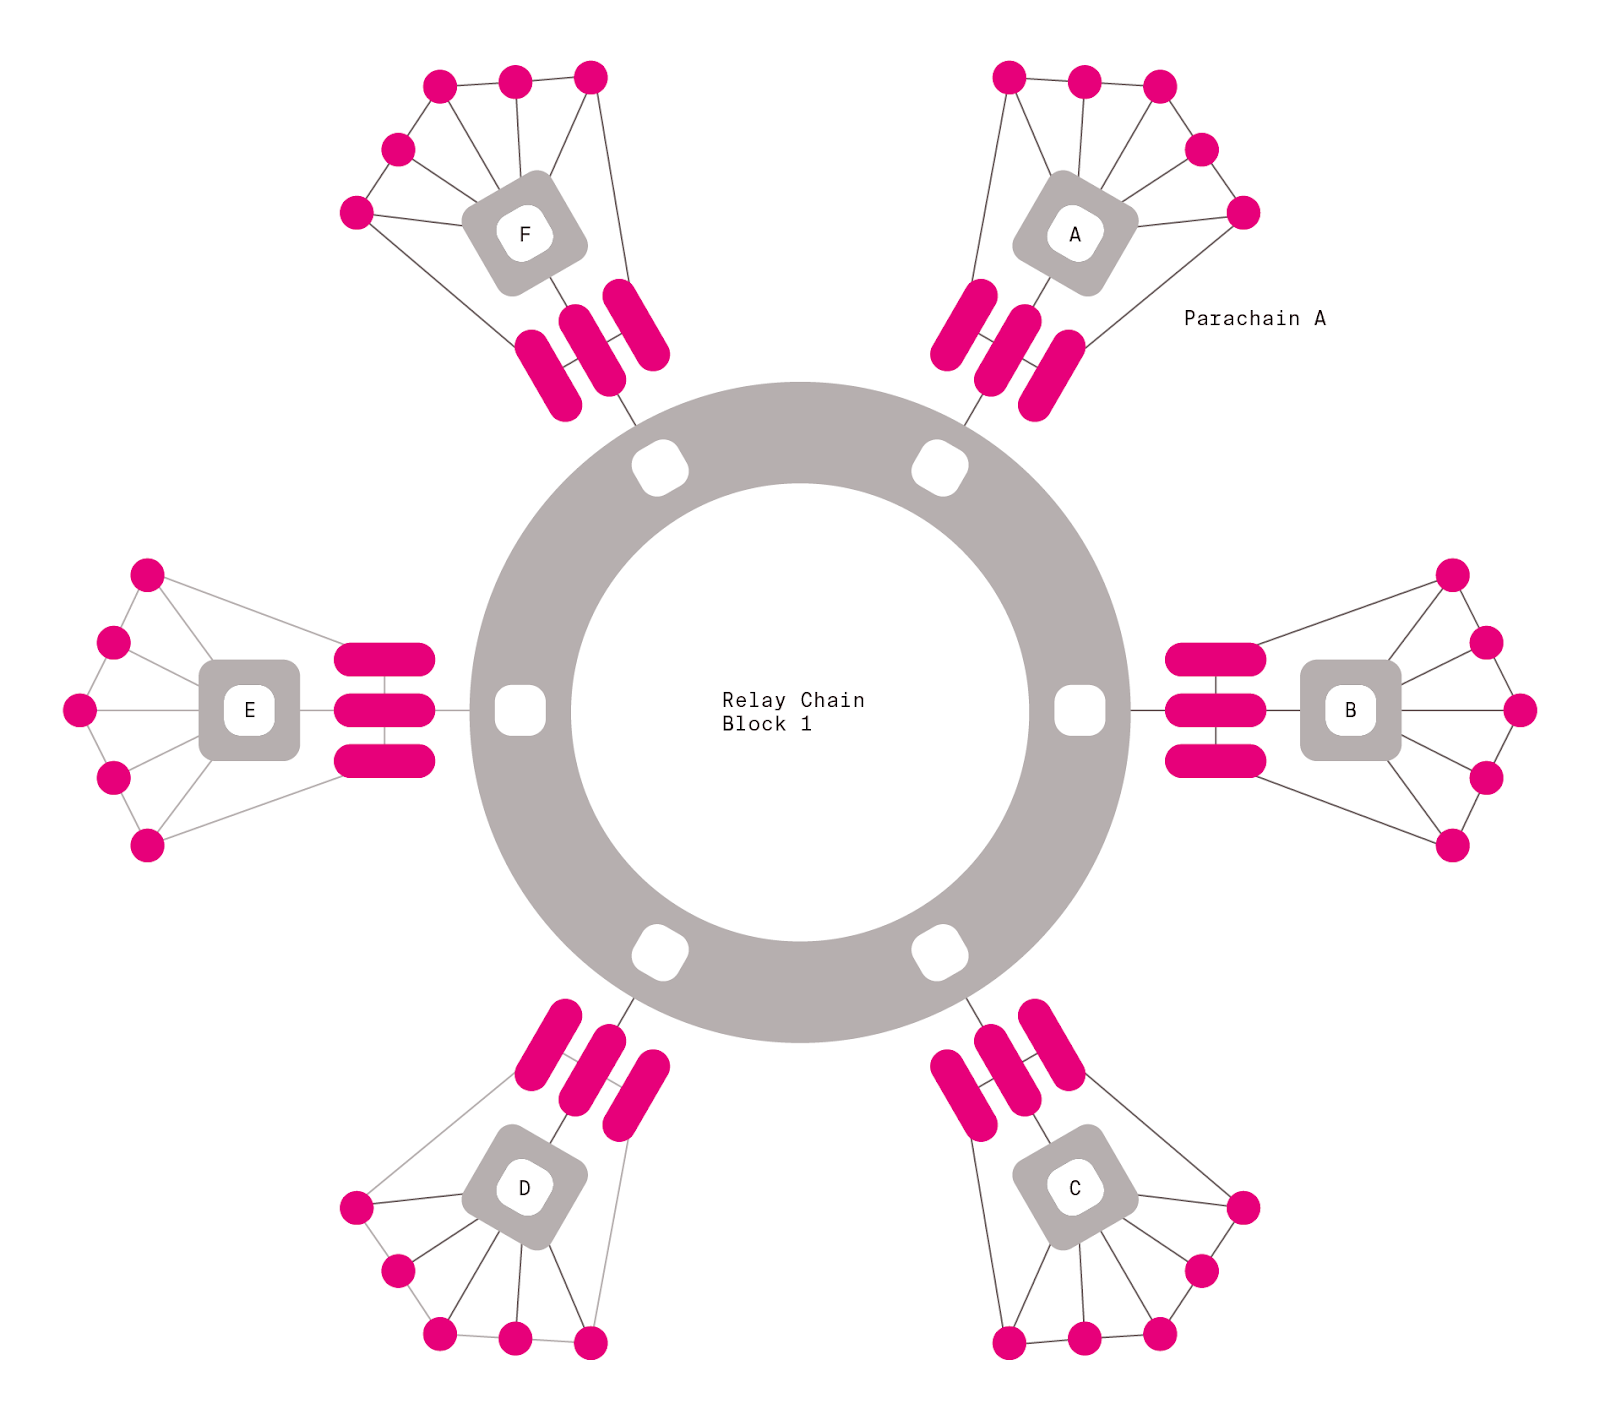
\includegraphics[width=0.4\linewidth]{polkadot_architecture.png}
  \caption{Polkadot's Architecture}
  \label{fig:polkadot_arch}
\end{figure}

Polkadot provides the bedrock “relay-chain” upon which a large number of validatable, globally-coherent dynamic data-structures may be hosted side-by-side (polkadot whitepaper)

In the Figure \ref{fig:polkadot_arch} you can see in the middle the relay chain that connects multiple parachains.

\subsection{Polkadot's protocol}

Briefly the Polkadot system consists of a single open collaborative decentralised network (relay chain), that interacts with many other external chains (para chains)(polkadot-overview). For the realy chain the internals of the parachians are not relevant, parachains need only to adhere to a specific interface. The relay chain then ensure that the parachain is trustable as a whole, not single nodes.

TODO explain roles and the protocol in general

\begin{enumerate}
  \item Each parachain:
        \begin{enumerate}
                \item collectors run full relay chain node to keep up the latest state
                \item build new block on top of this latest state and submit blocks to the parachain's validator
                \item parachian's validator produce the new relay chain block candidate
        \end{enumerate}
    \item validator block producing behaviour ...
    \item substrotocol to ensure data sharding
    \item managing of messagging between parachians
    \item validators submit votes to resolve forks and have a single head
\end{enumerate}

(from polkadot overview)

Explanation of the STATE TRANSITION FUNCTION

`Like any transaction-based transition system, Polkadot state changes via an executing ordered set of instructions, known as extrinsics`
(from polkadot overview)

Polkadot relay chain is divided in:
    1. Runtime -> contain the state transition logic, compiled into WASM and stored as part of the state (under well known keys), in this way the state transition logic can be upgraded
    2. Runtime environment / Client -> contian all the remaining blockchain relted stuff

QUESTION -> technically this section could require 100 pages, is it ok to explain here ONLY the relevant part to understand the next section?

\subsection{WASM in Polkadot}

% Runtime Interactions
`Polkadot’s state is changed by executing an ordered set of instructions(extrinsics)`

`For easy upgradability this Runtime is presented as a Wasm blob`

(from polkadot spec)

% MAYBE -> \subsubsection{Key features for an PAB}
\subsubsection{Usage a WAMS in Polkadot}
\paragraph{STF}

Talking about SUBSTRATE and how facilate the construction of the client and runtime

\paragraph{PVF}

talking about cumulus, PVF and PoV
% Somewhere I have to put also this -> \subparagraph{PoV}
\paragraph{SmartContracts}

talking about pallet-contracts that enable you to uplaod smart contracts onchain

\paragraph{SPREE}

???

\end{document}
